\documentclass[tikz,border=8pt]{standalone}
\usepackage{xcolor}
\usetikzlibrary{calc,arrows.meta,backgrounds,positioning}
\definecolor{bg}{HTML}{1B1F27}
\definecolor{fg}{HTML}{E6EDF3}
\definecolor{dim}{HTML}{9AA5B1}
\definecolor{ca}{HTML}{7BC47F}
\definecolor{cb}{HTML}{6EA8FE}
\definecolor{cc}{HTML}{F0C060}
\definecolor{cd}{HTML}{B39DDB}
\definecolor{ce}{HTML}{E5826F}
\begin{document}
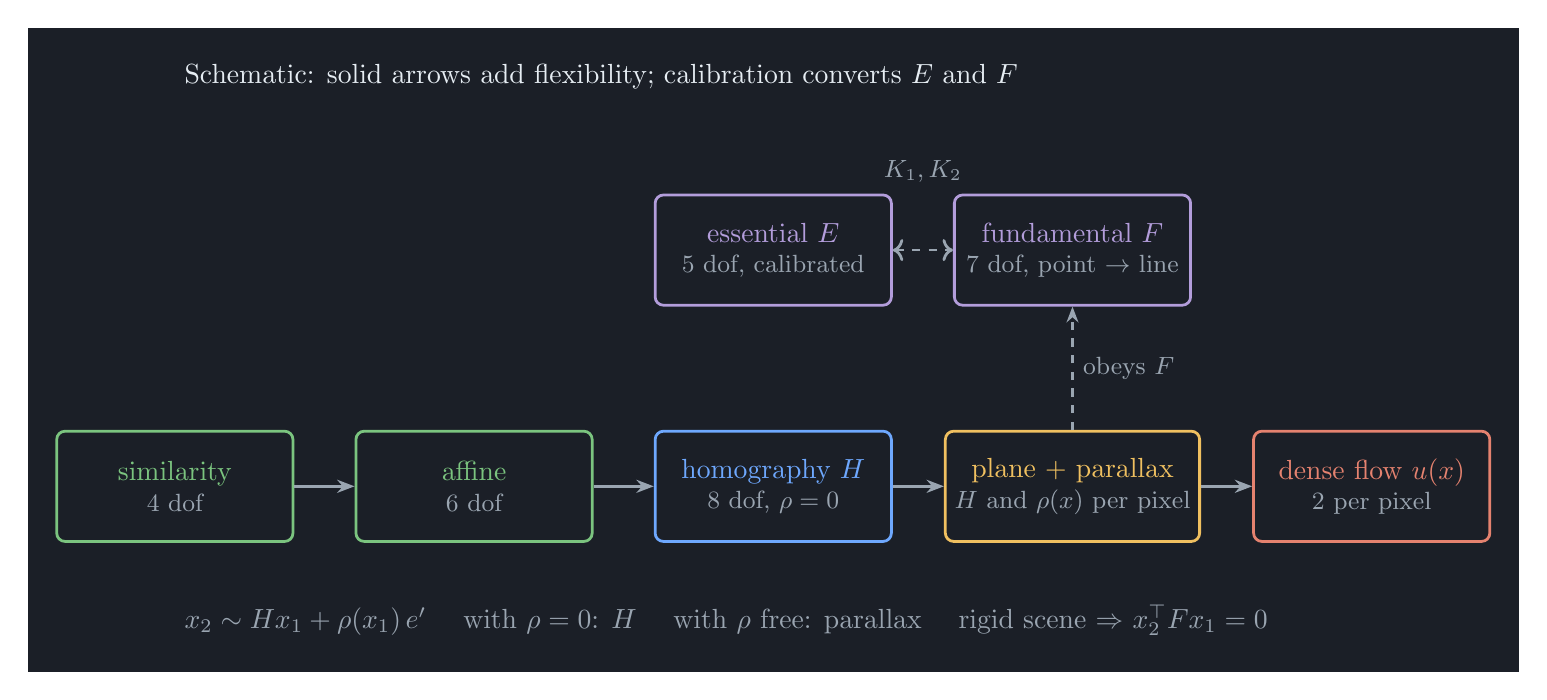
\begin{tikzpicture}[show background rectangle, background rectangle/.style={fill=bg}, inner frame sep=10pt, every node/.style={text=fg},
  box/.style={draw, rounded corners=3pt, line width=1pt, minimum width=3.0cm, minimum height=1.4cm, align=center, fill=bg},
  gen/.style={-{Stealth[length=2.2mm]}, line width=1.2pt, draw=dim, text=dim},
  obey/.style={-{Stealth[length=2mm]}, line width=1pt, dashed, dim}]
\node[box, draw=ca, text=ca] (S) at (0,0) {similarity\\[-1pt]{\small\color{dim}4 dof}};
\node[box, draw=ca, text=ca] (A) at (3.8,0) {affine\\[-1pt]{\small\color{dim}6 dof}};
\node[box, draw=cb, text=cb] (H) at (7.6,0) {homography $H$\\[-1pt]{\small\color{dim}8 dof, $\rho=0$}};
\node[box, draw=cc, text=cc] (P) at (11.4,0) {plane + parallax\\[-1pt]{\small\color{dim}$H$ and $\rho(x)$ per pixel}};
\node[box, draw=ce, text=ce] (U) at (15.2,0) {dense flow $u(x)$\\[-1pt]{\small\color{dim}2 per pixel}};
\node[box, draw=cd, text=cd] (E) at (7.6,3) {essential $E$\\[-1pt]{\small\color{dim}5 dof, calibrated}};
\node[box, draw=cd, text=cd] (F) at (11.4,3) {fundamental $F$\\[-1pt]{\small\color{dim}7 dof, point $\to$ line}};
\draw[gen] (S) -- (A); \draw[gen] (A) -- (H); \draw[gen] (H) -- (P); \draw[gen] (P) -- (U);
\draw[obey, <->] (E) -- (F);
\node[text=dim, font=\small] at (9.5,4) {$K_1,K_2$};
\draw[obey] (P) -- node[right, text=dim, font=\small] {obeys $F$} (F);
\node[anchor=west] at (0,5.2) {Schematic: solid arrows add flexibility; calibration converts $E$ and $F$};
\node[anchor=west, text=dim] at (0,-1.7) {$x_2\sim Hx_1 + \rho(x_1)\,e'$ \quad with $\rho=0$: $H$ \quad with $\rho$ free: parallax \quad rigid scene $\Rightarrow$ $x_2^{\top}Fx_1=0$};
\end{tikzpicture}
\end{document}
